\documentclass[11pt,a4paper]{article}


\usepackage{ctex}

\usepackage[margin=2.5cm]{geometry}
\usepackage{amsmath,amssymb}
\usepackage{enumitem}
\usepackage{xcolor}
\usepackage{titlesec}
\usepackage{fancyhdr}
\usepackage{tcolorbox}

\definecolor{accent}{RGB}{30,60,114}
\definecolor{notebg}{RGB}{245,248,255}
\definecolor{tipbg}{RGB}{255,249,230}

\titleformat{\section}{\Large\bfseries\color{accent}}{\thesection}{1em}{}
\titleformat{\subsection}{\large\bfseries\color{accent!80}}{\thesubsection}{1em}{}
\titleformat{\subsubsection}{\normalsize\bfseries\color{accent!60}}{\thesubsubsection}{1em}{}

\usepackage{graphicx}
\usepackage{hyperref}
\hypersetup{colorlinks=true,linkcolor=accent,urlcolor=accent!70}

\pagestyle{fancy}
\fancyhf{}
\fancyhead[L]{\small\textcolor{gray}{Attention Is All You Need}}
\fancyhead[R]{\small\textcolor{gray}{老奶奶通俗讲解}}
\fancyfoot[L]{\scriptsize\textcolor{gray}{Generated by \textbf{ScholarFlow} \textbar\ GitHub: \url{https://github.com/bcefghj/scholarflow}}}
\fancyfoot[R]{\scriptsize\textcolor{gray}{小红书: bcefghj \textbar\ \thepage}}

\newtcolorbox{notebox}{colback=notebg,colframe=accent!30,boxrule=0.5pt,arc=3pt}
\newtcolorbox{tipbox}{colback=tipbg,colframe=orange!40,boxrule=0.5pt,arc=3pt}

\begin{document}

\begin{center}
{\LARGE\bfseries 老奶奶通俗讲解}\\[0.5em]
{\large Attention Is All You Need}\\[0.3em]
{\normalsize Attention Is All You Need}
\end{center}

\vspace{1em}
\noindent\rule{\textwidth}{0.4pt}
\tableofcontents
\noindent\rule{\textwidth}{0.4pt}
\vspace{1em}

\section*{奶奶讲论文：Attention Is All You Need}

\subsection*{这论文是干啥的？（一句话版）}

来来来，奶奶跟你说啊，这篇论文就是教电脑怎么\textbf{更好地翻译各国语言}的。你想想，以前电脑翻译慢吞吞的，还翻得磕磕绊绊；这帮人整了个新法子，让电脑翻译又快又好，还特别能理解上下文——就是这篇论文干的事儿！

\vspace{0.5em}\noindent\rule{\textwidth}{0.4pt}\vspace{0.5em}

\subsection*{为什么要做这个研究？}

\subsubsection*{以前的方法有啥毛病？}

你们知道以前电脑是怎么学翻译的吗？它用的是一种叫\textbf{循环神经网络（RNN）}的东西。这名字听着吓人，奶奶给你打个比方：

想象你是一个抄书先生，要抄一本厚厚的书📖。可是你只能用一支钢笔，还必须\textbf{从第一页一个字一个字抄到最后一页}。为啥？因为你抄到第100页的时候，必须记得第99页写的啥——不能跳着抄啊！

这就是RNN的问题：

\begin{itemize}
  \item \textbf{必须一个词一个词顺序处理}，就像排队买火车票，不能好几个人同时排
  \item \textbf{距离远的词关系难捕捉}——就像隔了10页的内容，你记性不好就忘了联系起来
\end{itemize}

\subsubsection*{这篇论文的人想解决什么问题？}

Google这帮聪明孩子就想：\textbf{能不能让电脑像咱们聊天一样，同时"看见"整句话的所有词，然后一下子找出哪些词跟哪些词有关系？}

对啊！咱们人读句子的时候，眼睛一扫就知道"主语是哪个""动词是哪个"，不用一个字一个字硬记。电脑为啥不能这样呢？

于是他们整出了个新架构，叫\textbf{Transformer}，中文叫"变形金刚"——嘿嘿，挺贴切，它确实把翻译这事儿变得超级厉害！

\vspace{0.5em}\noindent\rule{\textwidth}{0.4pt}\vspace{0.5em}

\subsection*{奶奶给你讲明白核心方法}

\begin{figure}[htbp]
\centering
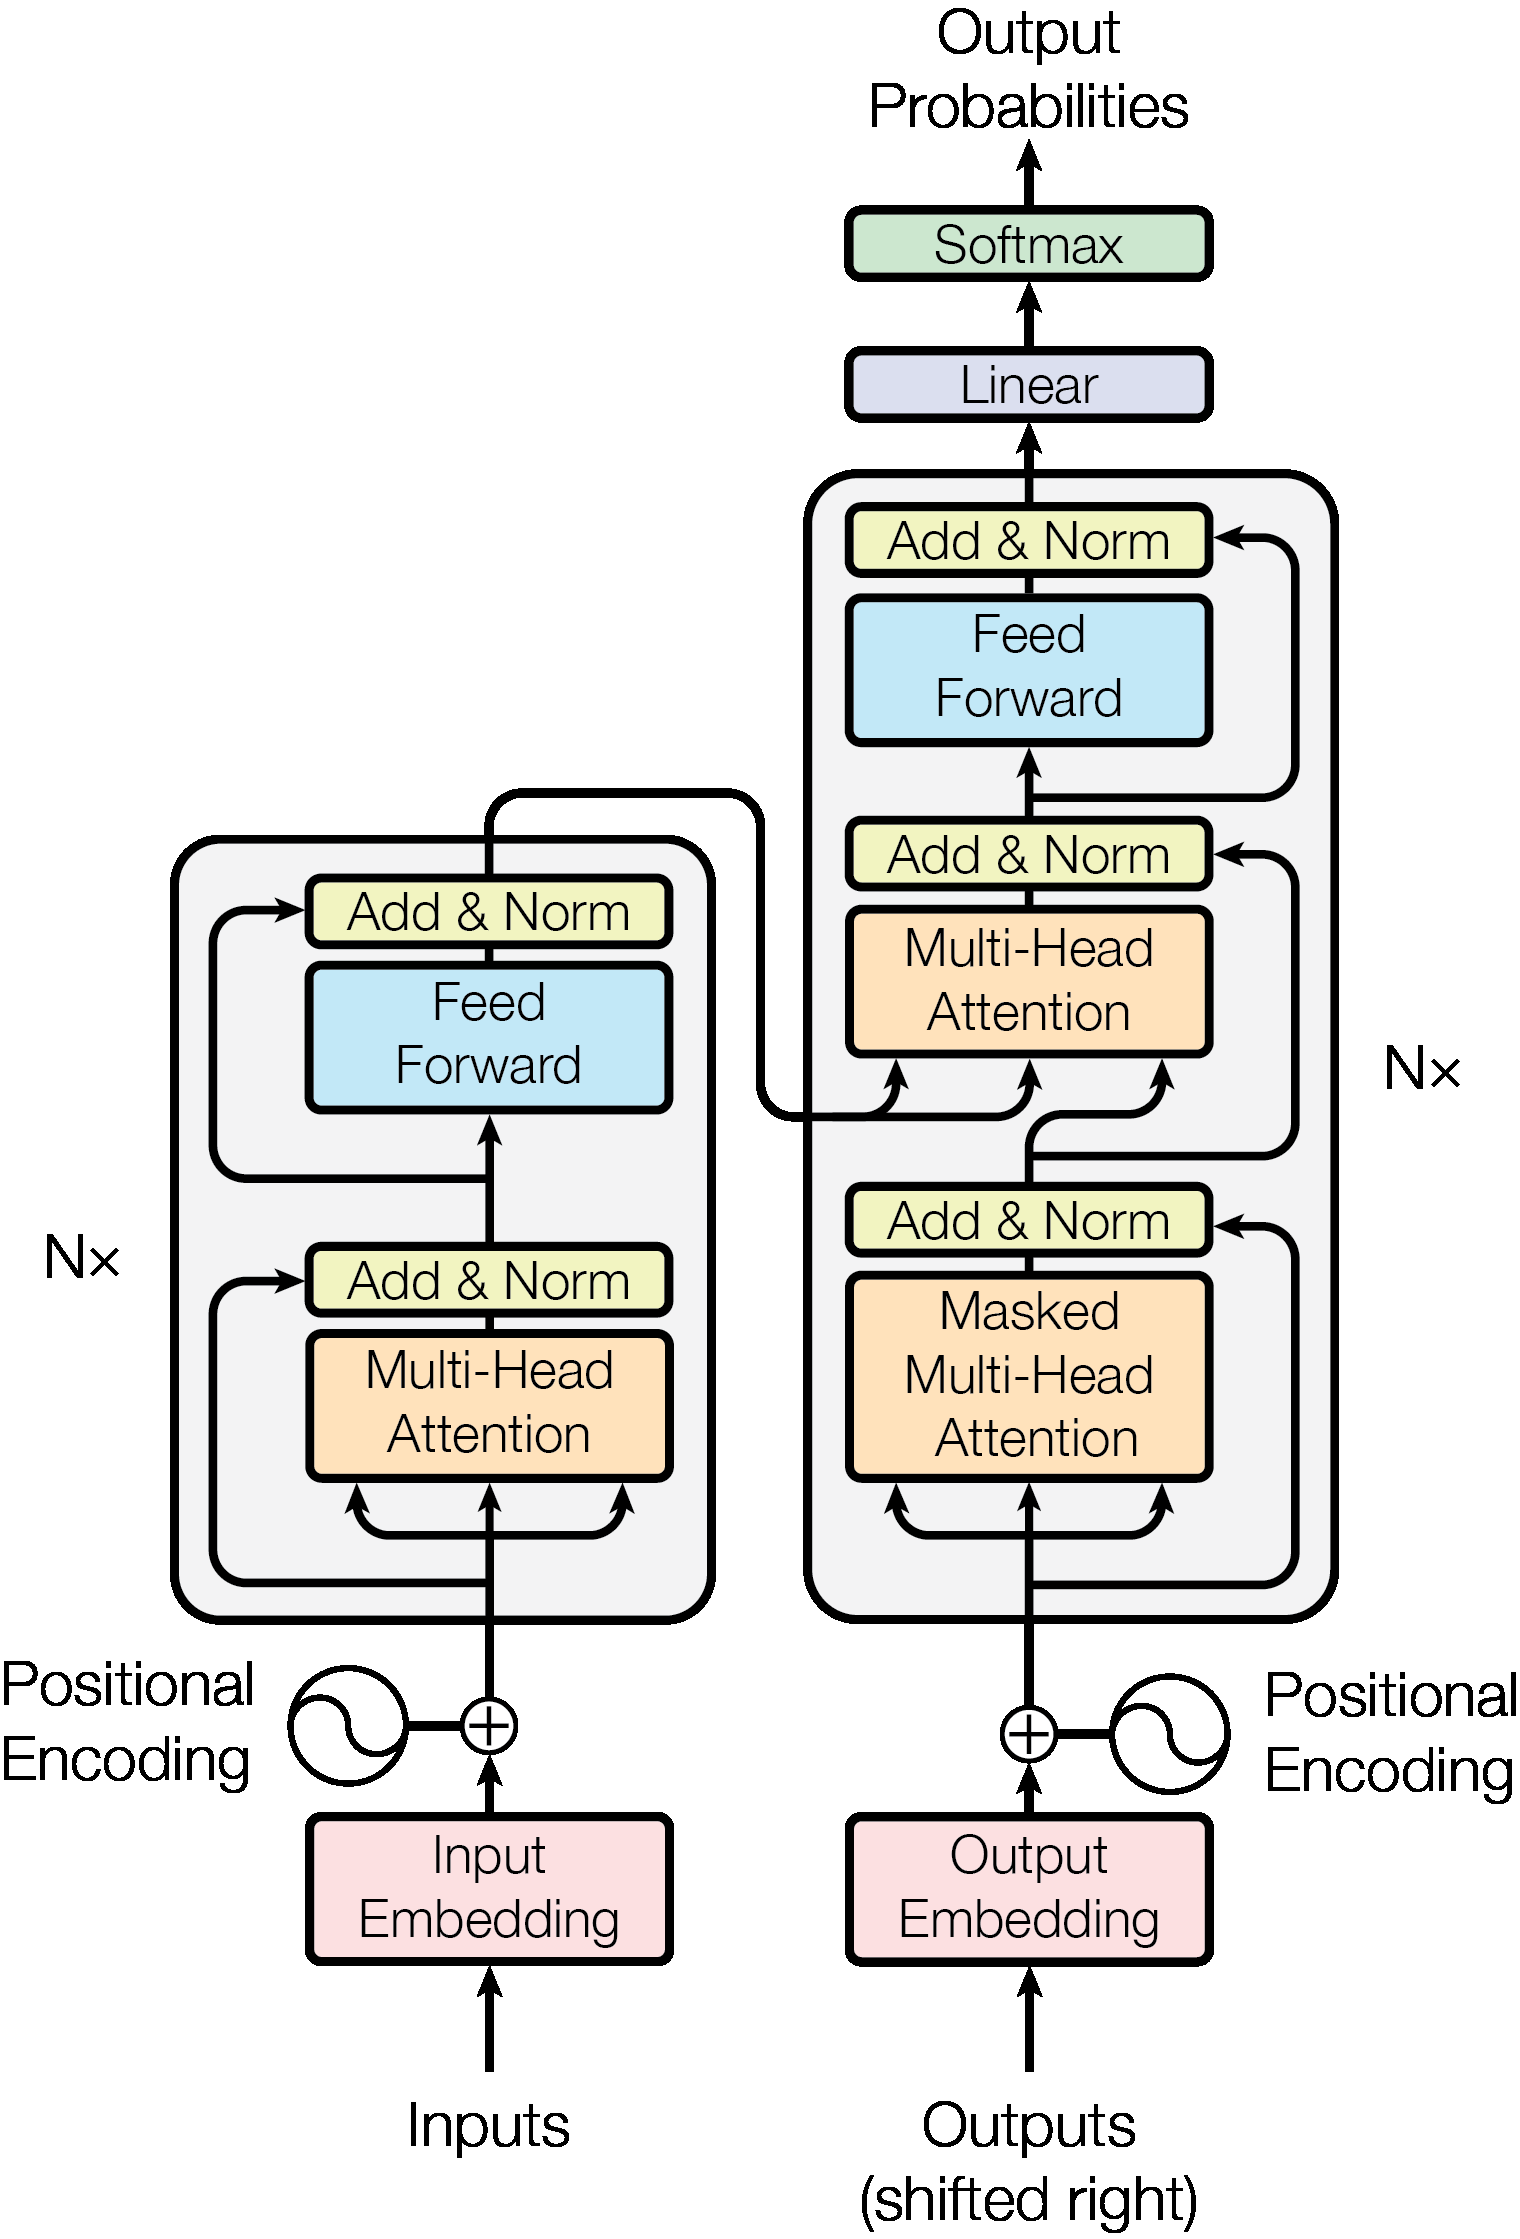
\includegraphics[width=0.8\textwidth]{fig1_p3.png}
\end{figure}

\subsubsection*{整个系统就像一个翻译工厂}

奶奶给你画个图📝（指着论文里的图1）：

这个Transformer啊，就像一个\textbf{翻译工厂}，分成两大部分：

\textbf{编码器（Encoder）}——就像一个阅读理解专家，先把原文"吃进去"，彻底搞懂每一句话的意思。

\textbf{解码器（Decoder）}——就像一个作家，根据专家的理解，用自己的话重新表达出来。

你想想中英文翻译班的老教授怎么工作的？他先\textbf{把整句英文读一遍}，搞懂意思；然后\textbf{闭眼组织语言}，用中文说出来。这不就是编码再解码的过程嘛！

\subsubsection*{最关键的"注意力机制"，就好比......}

好，奶奶现在要讲最核心的概念了！

\textbf{注意力机制（Attention）}是啥意思？奶奶给你打三个比方👵：

\paragraph{比喻1：老奶奶找东西}

咱们老年人记性不好，找东西的时候咋办？不是翻箱倒柜一个抽屉一个抽屉找——而是\textbf{眼睛一扫，脑子里一亮}：哦，那个东西应该在\textbf{显眼的地方}！

电脑的注意力机制就是这样：给它一句话，它不是傻傻地一个词一个词死记，而是\textbf{一下子"看"完全句，然后自动聚焦在最重要的词上}。

比如说"我家有一只黑色的可爱小猫"——电脑马上知道"小猫"是主角，"黑色的""可爱的"是修饰它的。\textbf{一下子抓住重点！}

\paragraph{比喻2：朋友聚会聊天}

你想想咱们一桌子人吃饭聊天👏。虽然嘈杂，但你跟旁边人说话时，\textbf{你会自动屏蔽其他声音，专注听你朋友说}——这不就是"选择性注意力"吗？

注意力机制就是这个道理：输入一堆词，它会自动判断"这个词跟那个词关系大"，然后重点处理关系大的。

\paragraph{比喻3：相亲大会配对}

哈哈，这个有意思！你把"查询（Query）"想成找对象的小伙子，"键（Key）"就是姑娘们的个人简介，"值（Value）"是姑娘本人的详细信息。

小伙子拿着自己的条件到处问："有没有和我兴趣相投的姑娘？"系统一匹配，发现A姑娘简历跟他最配，那就把A姑娘的资料重点推荐给他。\textbf{就是这么一个"相亲配对"的过程！}

\subsubsection*{"自注意力"更神奇——自己看自己}

\textbf{自注意力（Self-Attention）}是注意力机制的升级版。奶奶再给你打个比方：

自注意力就是让一句话\textbf{自己看自己内部的关系}。就像咱们读书的时候，眼睛看着"小猫"这个词，脑子里同时想着：\textit{"小猫"是主语，和后面的"抓老鼠"有关系，"黑色的"是修饰"小猫"的......}

奶奶读句子会\textbf{一边读一边思考}：这个词和前面那个词啥关系？有没有指代前面的东西？

Transformer的自注意力就是让电脑学会\textbf{"一边读一边想"}——这才是真正的理解啊！

\subsubsection*{多头注意力——八个脑袋一起想}

\textbf{多头注意力（Multi-Head Attention）}又是啥？

奶奶跟你说，咱们老年人看问题容易\textbf{片面}——看一个人只看长相，或者只看穿着。

可是电脑聪明啊，它有\textbf{8个"脑袋"同时看一个问题}！

\begin{itemize}
  \item 脑袋1专门看\textbf{语法结构}：主语在哪、谓语在哪
  \item 脑袋2专门看\textbf{指代关系}：这个"他"指的是谁
  \item 脑袋3专门看\textbf{语义相似}："快乐"和"高兴"是近义词
  \item 脑袋4专门看\textbf{位置关系}：谁在谁前面
  \item ……一共8个！
\end{itemize}

然后8个脑袋各自汇报，\textbf{最后汇总成一个全面、准确的理解}！

\begin{figure}[htbp]
\centering
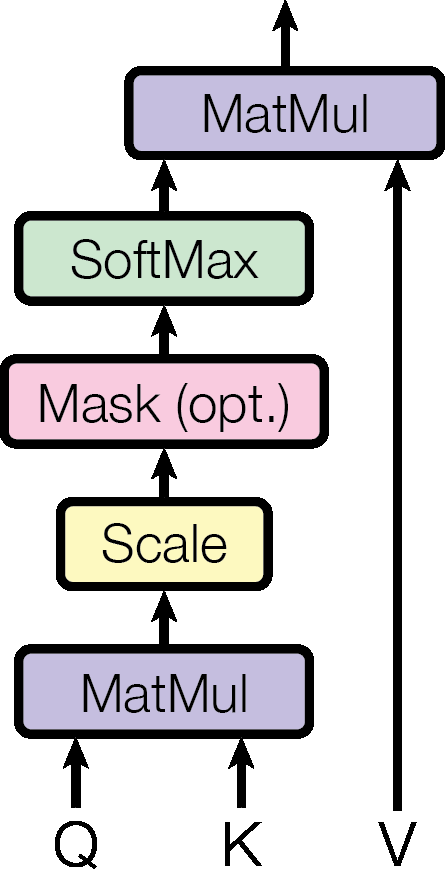
\includegraphics[width=0.8\textwidth]{fig2_p4.png}
\end{figure}

\subsubsection*{位置编码——让电脑知道"谁先谁后"}

有个问题啊：注意力机制虽然能抓住词与词的关系，但它\textbf{不知道词在句子里哪个位置}！

"狗咬人"和"人咬狗"，词都一样，意思完全相反。电脑咋知道区分？

这里论文用了一个很巧妙的办法——\textbf{位置编码（Positional Encoding）}。

奶奶给你解释：想象每个词不只是自己来，还有一个\textbf{"座位号"}跟着它。

就像宴会上，主桌放1号椅子、2号椅子......每个来宾都有固定座位。电脑看到"狗"的座位号是第1个，"咬"是第2个，"人"是第3个——它就知道这是在说"狗"先动作"咬"，"人"是承受者。

论文用\textbf{正弦波函数}来生成这些位置信息，听着复杂，其实就是给每个位置发一个独一无二的"暗号"——聪明的设计！

\vspace{0.5em}\noindent\rule{\textwidth}{0.4pt}\vspace{0.5em}

\subsection*{实验结果怎么样？}

\subsubsection*{翻译比赛，Transformer拿了冠军🏆}

Google这帮人做了两组实验：

\textbf{英译德}：Transformer得了\textbf{28.4分}（BLEU分数，越高越好），比之前最好的成绩还高2分多！你要知道，在翻译任务里提高0.5分都很难，何况2分！

\textbf{英译法}：得了\textbf{41.8分}，刷新了单模型的世界纪录！

\subsubsection*{最亮眼的是：又快又省！}

以前训练一个翻译模型要好几天甚至几周。他们这个大模型，\textbf{只用8块GPU训练3.5天}——跟现在的AI训练动不动要几个月比起来，简直是神速！

而且训练成本大大降低。论文里有个表格对比，算了一下用了多少"计算力"——Transformer用的最少，但效果最好！\textbf{又快又好又省钱，你说是不是很牛？}

\subsubsection*{还能用来做句子的语法分析！}

更有意思的是，这模型不只能翻译，还能\textbf{分析英文句子的语法结构}！

比如给它一句"The law will never be perfect"（法律永远不会完美），它能告诉你：这句话的主语是"law"，谓语是"will be"，还有各种从句、修饰语等等。

而且只给它很少的训练数据（4万句），效果就能超过很多老牌的语法分析工具！\textbf{举一反三，触类旁通}——这说明Transformer学到的不是死知识，而是真正的"语言能力"。

\vspace{0.5em}\noindent\rule{\textwidth}{0.4pt}\vspace{0.5em}

\subsection*{这论文为什么牛？}

\subsubsection*{第一，彻底颠覆了传统！🔄}

以前的翻译模型都要靠\textbf{循环神经网络（RNN）}——必须一个词一个词顺序处理，就像只能走不能跑的走路人。

Transformer直接把这个"跑步"都不让用的RNN\textbf{彻底抛弃了}！它靠注意力机制，\textbf{一步到位，同时处理所有词}。

这在AI领域相当于什么？相当于从绿皮火车直接跳到高铁——\textbf{质的飞跃！}

\subsubsection*{第二，效率大幅提升！⚡}

由于可以\textbf{并行处理}（大家一起来，不用排队），训练时间从几天缩短到几小时。Google论文里说，用8块GPU训练12小时就能搞定一个模型！

这对于实际应用太重要了——以前训练个模型要好几天，万一效果不好要调整，又得重来，时间全耗在这儿了。现在又快又灵活！

\subsubsection*{第三，长距离依赖问题解决了！🌟}

以前RNN最大的毛病就是：离得远的词，它记不住关系。就像你跟奶奶说"我小时候住的那个房子前面有棵大树，树上有只猫......"——说到后头，你可能忘了开头"我小时候住的那个房子"是主语！

Transformer的注意力机制让\textbf{任意两个词之间都可以直接"对话"}——不管它们在句子中隔了多远！

论文里还给了一些可视化例子，比如"making...more difficult"这个搭配，虽然中间隔了好多词，但注意力机制能准确地把它们联系起来。\textbf{这才是真正的"理解"啊！}

\vspace{0.5em}\noindent\rule{\textwidth}{0.4pt}\vspace{0.5em}

\subsection*{一句话记住它}

\begin{quote}
\textit{\textbf{Transformer不排队，全靠"注意力"一眼扫完全场！}}
\end{quote}

\vspace{0.5em}\noindent\rule{\textwidth}{0.4pt}\vspace{0.5em}

\subsection*{奶奶的小课堂：关键概念速查}

\begin{center}
\begin{tabular}{|l|l|}
\hline
术语 & 大白话解释 \\
\hline
\textbf{Transformer} & "变形金刚"——一种新的AI模型架构，专门处理序列数据（比如翻译句子），完全靠注意力机制，不用老式的循环网络 \\
\hline
\textbf{注意力机制（Attention）} & 就像老奶奶找东西，眼睛一扫就知道重点在哪，不用一个一个翻——电脑处理词的时候自动聚焦最重要的词 \\
\hline
\textbf{自注意力（Self-Attention）} & 让一句话自己看自己内部的关系，比如一边读"他"一边想"他指的是谁" \\
\hline
\textbf{多头注意力（Multi-Head Attention）} & 8个"脑袋"同时看问题，各有分工，最后汇总意见——集思广益看问题更全面 \\
\hline
\textbf{编码器（Encoder）} & 翻译工厂的"阅读理解部"——先把输入的句子彻底搞懂 \\
\hline
\textbf{解码器（Decoder）} & 翻译工厂的"输出部"——根据理解生成新的句子 \\
\hline
\textbf{Query（查询）、Key（键）、Value（值）} & 想象相亲大会：Query是找对象的小伙子，Key是姑娘简历，Value是姑娘本人——匹配上了就把姑娘推荐给你 \\
\hline
\textbf{位置编码（Positional Encoding）} & 给每个词发个"座位号"，让电脑知道谁在谁前面——解决"狗咬人"和"人咬狗"的顺序问题 \\
\hline
**BLEU分数 & 翻译质量的评分，满分是100，越高越好——就像作文比赛的得分 \\
\hline
\textbf{RNN（循环神经网络）} & 老式模型，必须一个词一个词顺序处理——就像只能排队的绿皮火车 \\
\hline
\end{tabular}
\end{center}

\vspace{0.5em}\noindent\rule{\textwidth}{0.4pt}\vspace{0.5em}

奶奶讲完了！👵✨

这Transformer啊，虽然是2017年的老论文了，但它奠定了现在所有大语言模型的基础——ChatGPT啊、Claude啊，都是它的"后代"！所以这篇论文可以说\textbf{改变了整个AI世界}。

你们回去好好想想这个"注意力机制"——生活中处处都有注意力，学会聚焦重点，咱们老年人也能跟上时代！

\end{document}